\section{Interaction of particles with matter}
\label{sec:interaction_particle_matter}

\subsection{Energy loss through ionisation*}
We can quantify the energy loss of a particle traversing through the detector, by looking at the average rate of energy lost per unit distance.


For an incident particle of charge $ze$ with mass $M\gg m_e$, losing energy by ionising atomic electrons in a material with atomic number $Z$ we can use the Bethe-Bloch equation:

\begin{equation}
\label{eq:bethebloch}
<\frac{dE}{dx}>\approx -2C\frac{m_ec^2Zz^2}{\beta^2A}\rho\left[\frac{1}{2}\log\frac{2m_ec^2\beta^2\gamma^2T_{\rm max}}{I^2}-\beta^2-\frac{\delta(\beta\gamma)}{2}\right]
\end{equation}
with \[C=2\pi N_A\frac{e^2}{4\pi\epsilon_0m_ec^2}.\] 
$I$ is the mean ionisation potential ie $h<\nu_e>$ (given by $\sim10Z$~eV for $Z>20$), $\rho$ is the density of the material, $\delta(\beta\gamma)$ is a density correction term because the incoming particle can polarise the medium, and $T_{\rm max}$ is the maximum energy transfer in a single collision given by
\[
T_{\rm max}=\frac{2m_ec^2\beta^2\gamma^2}{[1+2\gamma m_e/M +(m_e/M)^2].}
\]
For $\frac{\gamma m_e}{M}<<1$, $T_{\rm max}$ can be simplified to
\[
T_{\rm max}\sim2\gamma^2\beta^2m_ec^2.
\]

\paragraph{Important points:}
\begin{itemize}
\item Energy loss proportional to $\frac{1}{\beta^2}$ at low speeds
\item Relativistic effects result in a slow rise at higher speeds
\item Minimum energy loss occurs (``minimum-ionising'') for $\sim (3-4)\beta\gamma$ and features largely independent of material
\end{itemize}

\subsection{Energy loss through radiation*}
Energy loss by radiation also known as ``Bremsstrahlung'' or breaking radiation occurs when a relativistic charged particle changes direction due to the influence of the field of the charged nuclei of the material. Now you should know that the change of direction, ie acceleration of a charged particle, results in the production of EM waves. In this case the energy emitted per unit length is given by
\begin{equation}
\frac{dE}{dx}\propto \frac{E}{m^2},
\end{equation}
where $m$ is the rest mass of the charged particle. This means that Bremsstrahlung energy losses are much more prominent for electrons than for pions or muons. We can write the energy lost per unit distance as
\begin{equation}
\frac{dE}{dx}=-\frac{E}{X_{0}},
\end{equation}
where $X_0$ depends on the material composition and the charge and mass of the incoming particle. We typically define $X_0$ for electrons. We therefore have that
\begin{equation}
E=E_0e^{-x/X_0},
\end{equation}
where $E_0$ is the initial energy of the electron.
It is evident that $X_0$ denotes the mean distance over which a relativistic electron loses $E_0/e$ of its energy. The CMS detector uses lead tungstate crystals (PbWO$_4$) which have $X_0=0.89$~cm.

The fact that electrons radiate a lot more energy as they are deflected (accelerated) compared to say protons, means that building circular accelerators instead of linear accelerators for electrons, has its positives and negatives. The benefit of a circular accelerator is that you can save space (and money) by being able to cycle the beam in a given ring, increasing its energy as the beam circulates many many times, without having to build a very long accelerator. However the downside is that given electrons radiate away a large amount of energy when bending in a circular orbit, you need to make sure you supply more energy each time which in turn also costs money.

Considering both loses due to ionisation and Bremsstrahlung we have
\begin{equation}
\frac{dE}{dX}(\rm total)=\frac{dE}{dX}({\rm ionisation})+\frac{dE}{dX}({\rm bremsstrahlung})
\end{equation}

For typical electron energies produced in colliders $E_{e}\sim 1-100$~GeV (ie $\gg10$~MeV), therefore Bremsstrahlung emission dominates as shown in the figure below.
\begin{center}
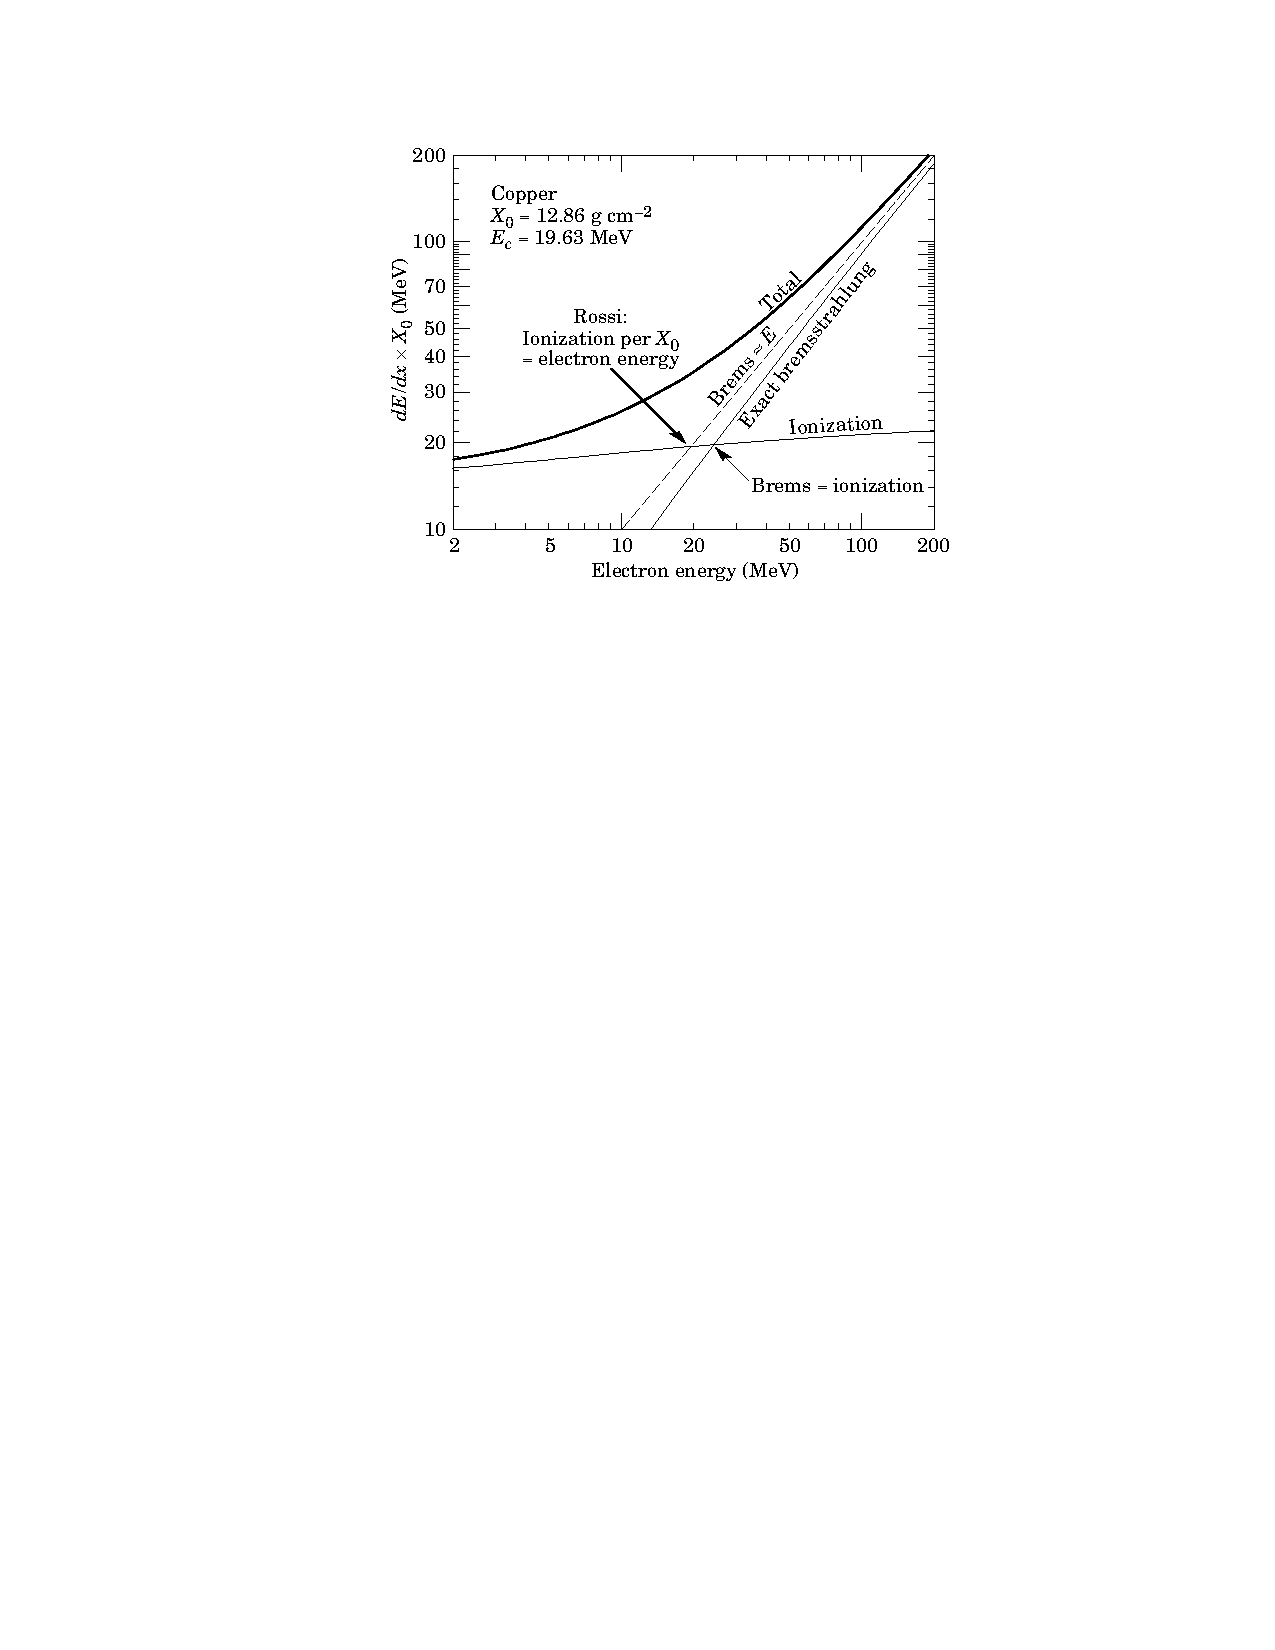
\includegraphics[width=0.6\textwidth]{fig/detector/e_energy_brem_vs_ion.pdf}
\end{center}

\subsection{Photon interactions with matter*}
Energies of photons relevant at most particle physics experiments $\gg10$~MeV.
At these energies pair production in the presence of the EM field of the charged nuclei dominate. At lower energies, Compton-scattering and the photo-electric effect dominate.
\begin{center}
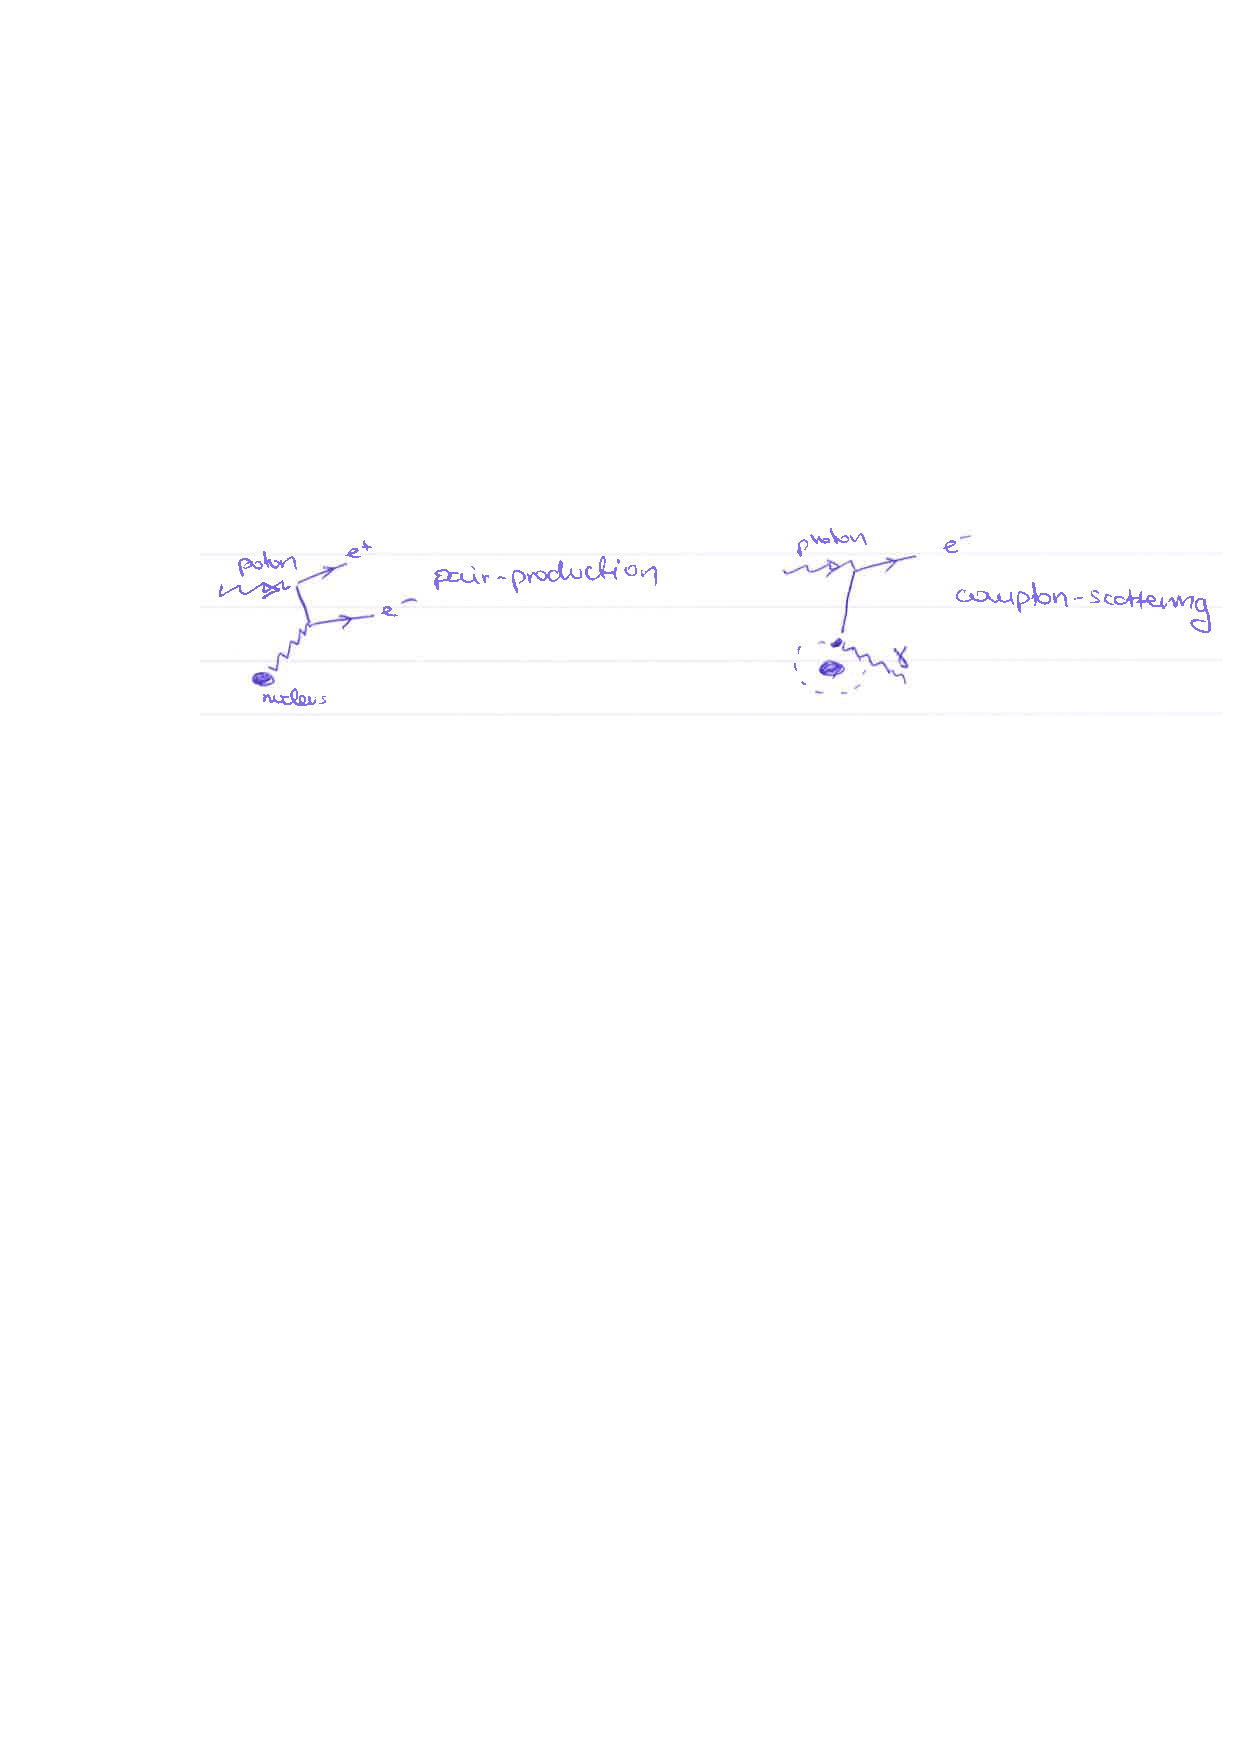
\includegraphics[width=0.95\textwidth]{fig/detector/photon_interactions.pdf}
\end{center}
Pair production has an energy threshold of $E_{\gamma}\geq 2m_{e}\sim1$~MeV. Below this energy, photons will lose energy via Compton scattering.
\begin{center}
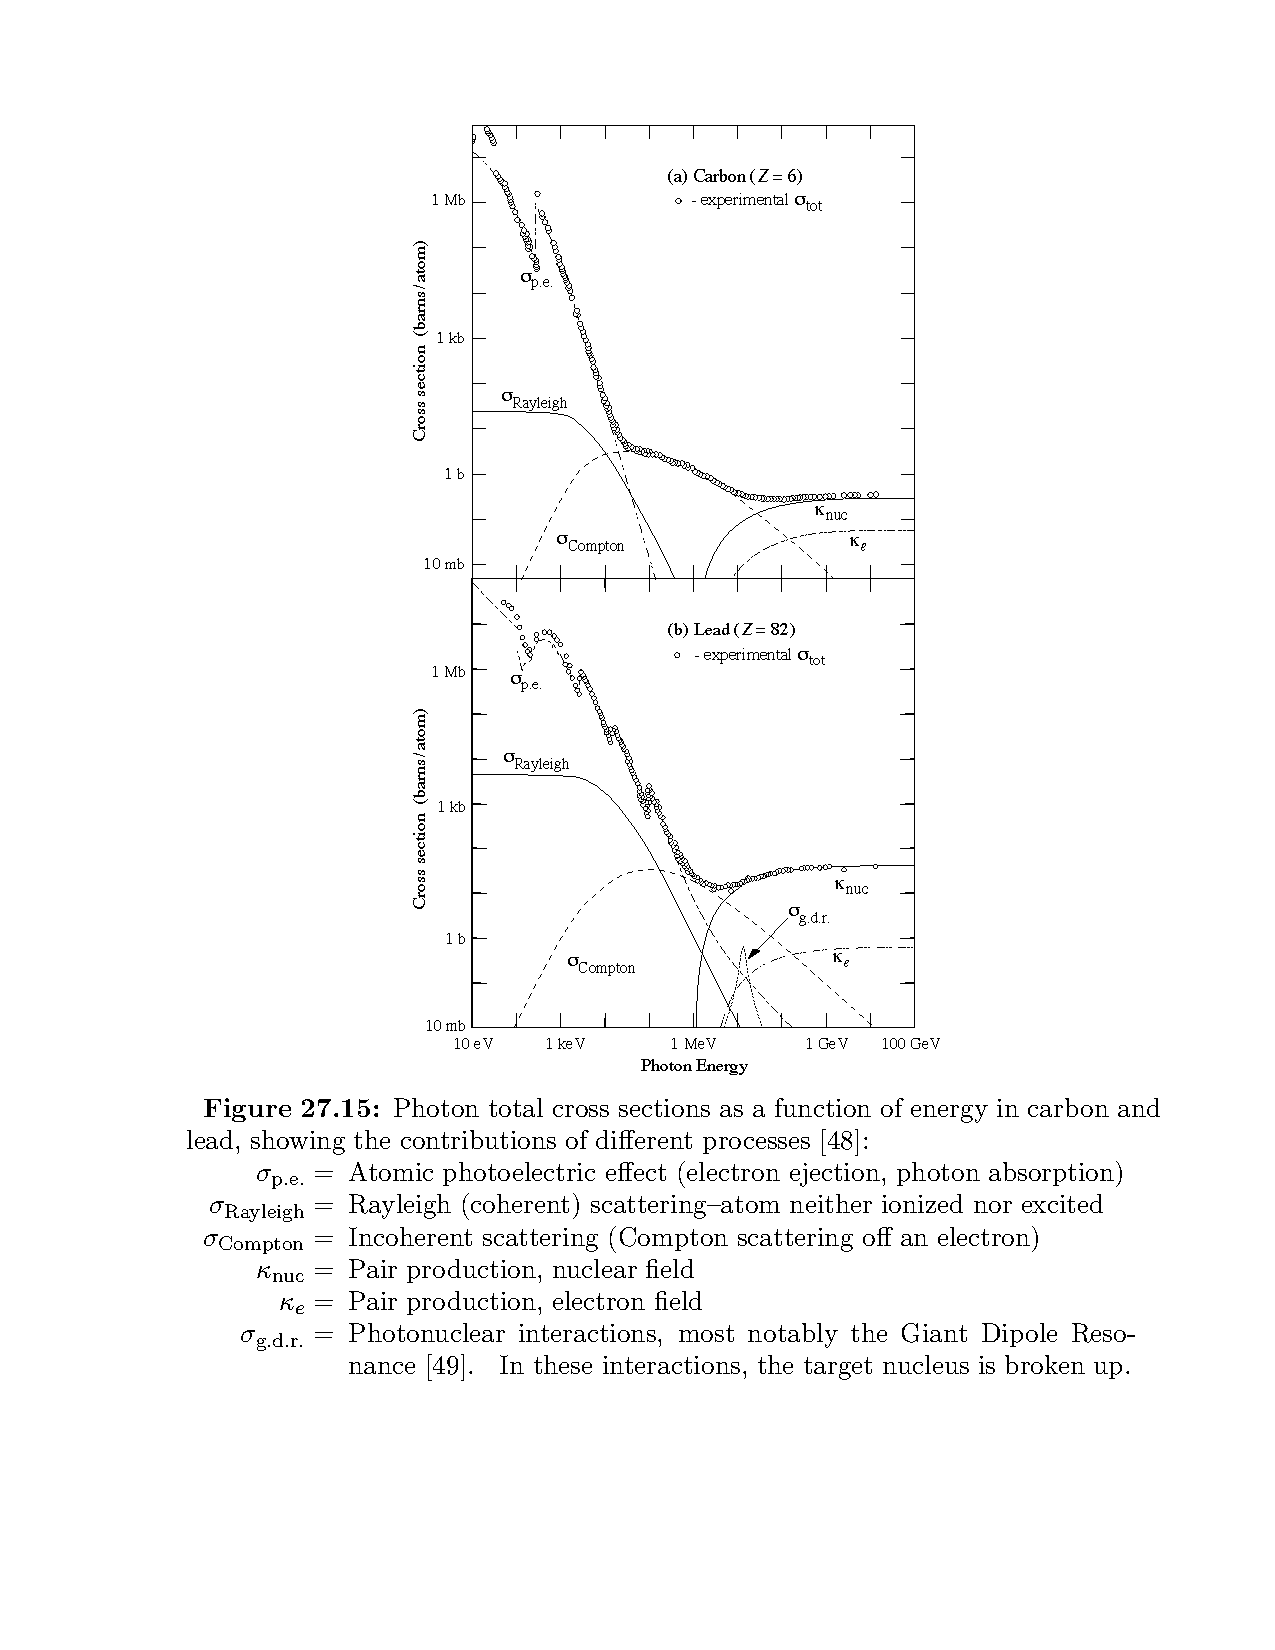
\includegraphics[width=0.90\textwidth]{fig/detector/photon_interactions_pdg.pdf}\\\tiny{Source:Particle Data Group}
\end{center}

\subsection{Electromagnetic showers*}
Incident electron or photons on thick material produce a cascade of EM processes through a chain of Bremsstrahlung and pair-production. A simplified picture is given below:
\begin{center}
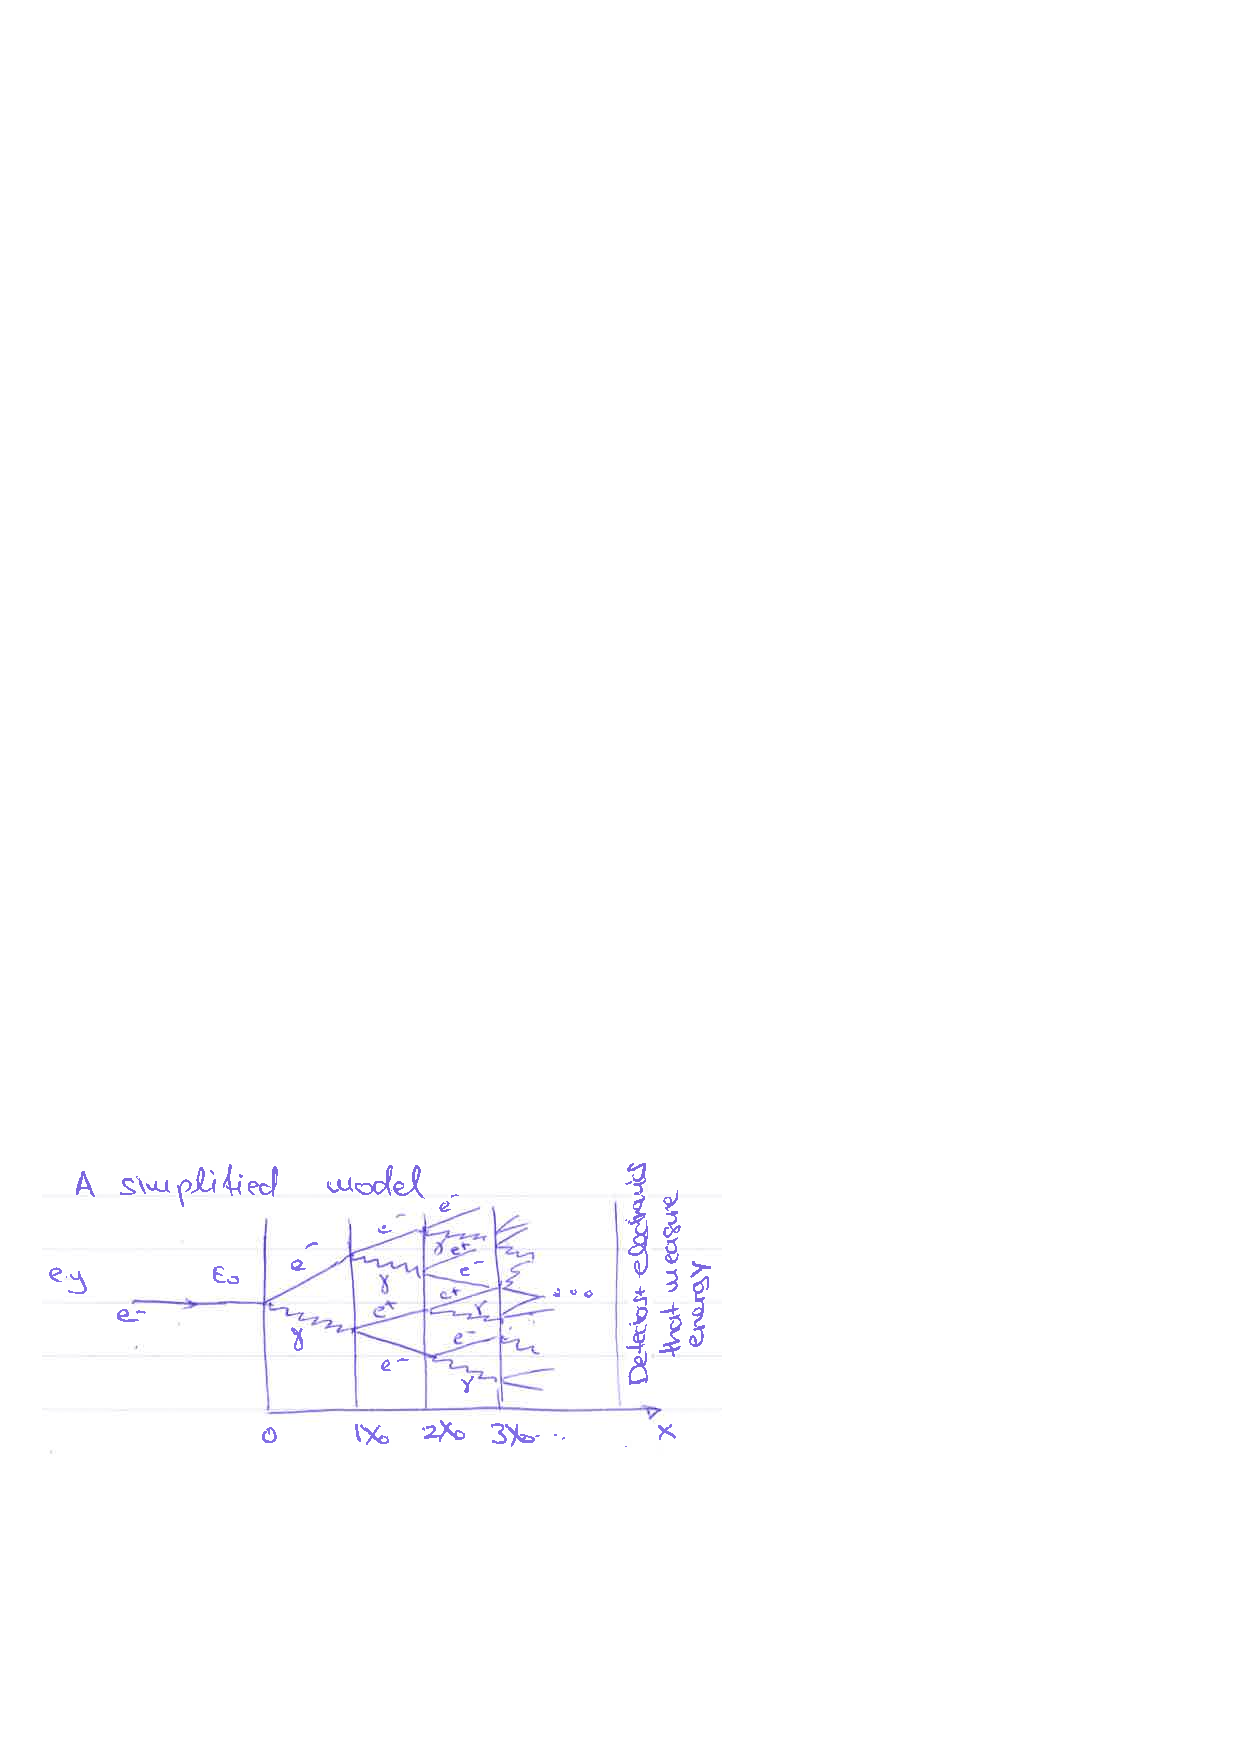
\includegraphics[width=0.90\textwidth]{fig/detector/em_shower.pdf}
\end{center}
In this simplified model, an interaction occurs every $X_0$. Assume radiation length of Bremsstrahlung and of pair-production is the same (in reality $\sim25\%$ different). 
Number of particles grows as $2^n$ where n is the integer number of radiation lengths. Energy per particle falls at each step as $E_02^{-n}$.
When electron energy falls below a critical level energy loss via ionisation dominates. Photons on the other hand loose energy via compotn scattering until the absorbed via the photoelectric effect.

Such detectors measure the energy of photons and electrons produced from the collision or from the decay of particles. These are called Electromagnetic Calorimeters (ECAL).
\subsection{Hadronic showers*}
Hadrons as as $\pi^{\pm}$, $p$, $n$ can interact with nucleons in nucleus via te strong force. So in a dense material we can have:
\[\pi^-+p\to n+\pi^0\]
ie in incoming pion on the proton of a dense material will interact via the strong force and produce a $\pi^0$ and a $n$. The $n$ will cause a subsequent strong interaction causing a hadronic shower in complete analogy to the EM shower. The $\pi^0$ will decay to a pair of photons which will initiate an EM shower. Therefore the situation with hadronic interactions with dense material is more complicated as you can get a combination of hadronic and EM showers.
In contrast to EM showers, the mean distance for a hadronic shower is called in interaction length $\lambda$ and has typical sizes of $\mathcal{O}(10)$~cm compared to interaction lenghs of $\mathcal{O}(1)$~cm. Detectors meant to measure energies of hadrons are called hadronic calorimeters (HCAL) and due to the larger showers, they tend to be larger than ECALs.

\subsection{Cherenkov radiation*}
A charged particle that moves in a medium with a velocity larger than the velocity of the speed of light in this medium (ie $v>c/n$ where $n$ is the refractive index of the medium), will emit a cone of light very much like the cone of sound of a sonic boom of an aircraft breaking the sound barrier (or like the ripples a duck produces as it swims in the pond)
\begin{center}
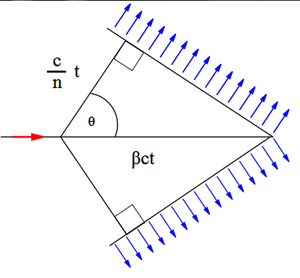
\includegraphics[width=0.45\textwidth]{fig/detector/cherenkov_angle.png}
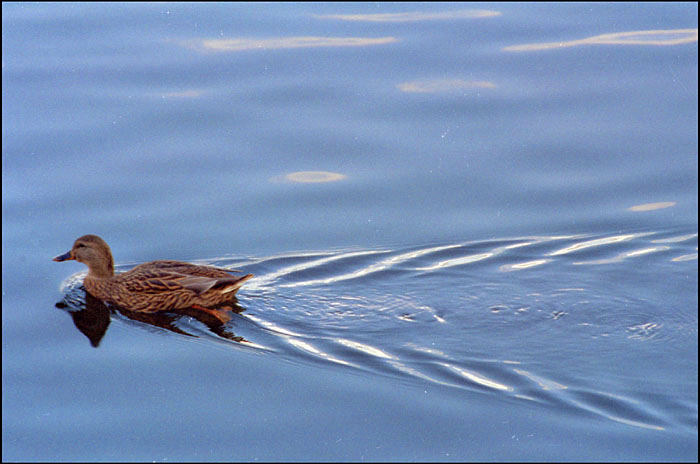
\includegraphics[width=0.45\textwidth]{fig/detector/duck_angle.png}
\end{center}
So photons are emitted at an angle $\theta_c$ given by 
\begin{equation}
\label{eq:cherenkov_angle}
\cos\theta_{C}=\frac{1}{n\beta}
\end{equation}
By placing a gas or liquid volume in path of the particle and surround this volume by photon detectors, the resulting Cherenkov photons form a ring. We call these detectors Ring Imaging Cherenkov (RICH) detectors. 
\begin{center}
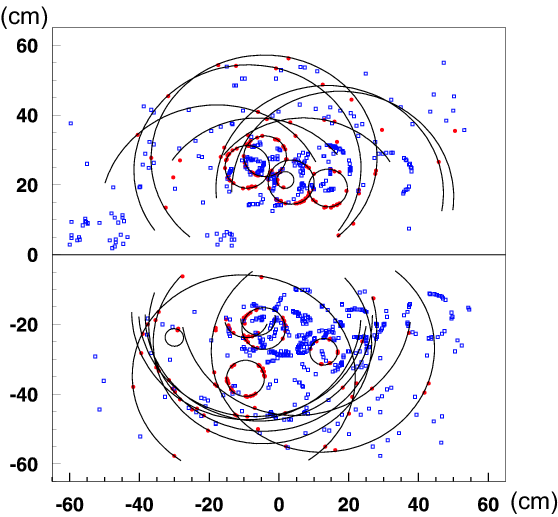
\includegraphics[width=0.75\textwidth]{fig/detector/rich_1_rings.png}
\end{center}
Measuring the Cherenkov angle allows to determine the speed of the particle. Combined with a measurement of the momentum of the particle, we can therefore determine very accurately the mass and hence the type of particle. An important point to remember and which also stems from Eq.~\ref{eq:cherenkov_angle}, is that Cherenkov radiation is only emitted if $\beta>\frac{1}{n}$. Additionally, as the particle's speed increases, $cos\theta_{C}$ approaches $\frac{c}{n}$ asymptotically. Thus the ability to determine the speed of the particle becomes more and more difficult as the ring size changes less and less. A solution is to have two RICH detectors with materials of different $n$, in order to have good resolution for a large range of particle speeds.
\begin{center}
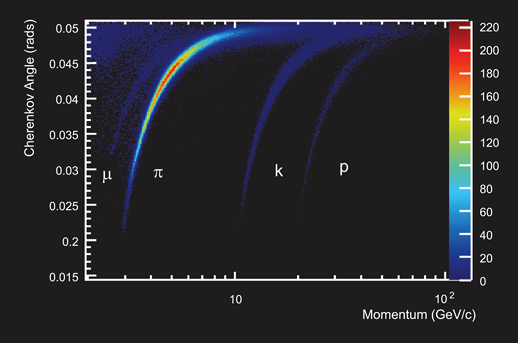
\includegraphics[width=0.75\textwidth]{fig/detector/lhcb_cherenkov_vs_momentum.png}
\end{center}


%%%In order to detect a particle it must interact with the material of the detector and transfer energy in some recognisable fashion.
%%%\paragraph{Particle detection occurs via the energy loss of particles through the material they traverse.}
%%%
%%%\paragraph{Possibilities}
%%%\begin{itemize}
%%%\item[(i)] EM charged particles $\rightarrow$ Ionisation, Bremsstrahlung$^*$, Cherenkov
%%%\item[(ii)] Hadrons $\rightarrow$ Nuclear interactions$^*$ (equivalent to ones above the involving the strong force)
%%%\item[(iii)] Photons $\rightarrow$ Pair production$^{**}$, Photoelectric effect, Compton effect
%%%\end{itemize}
%%%$^{(*)}$ Cause a shower of particles (see later).\newline
%%%$^{(**)}$ Total energy loss via a single interaction converting into charged particles.\newline
%%%Some examples of what these processes look like:
%%%
%%%\begin{center}
%%%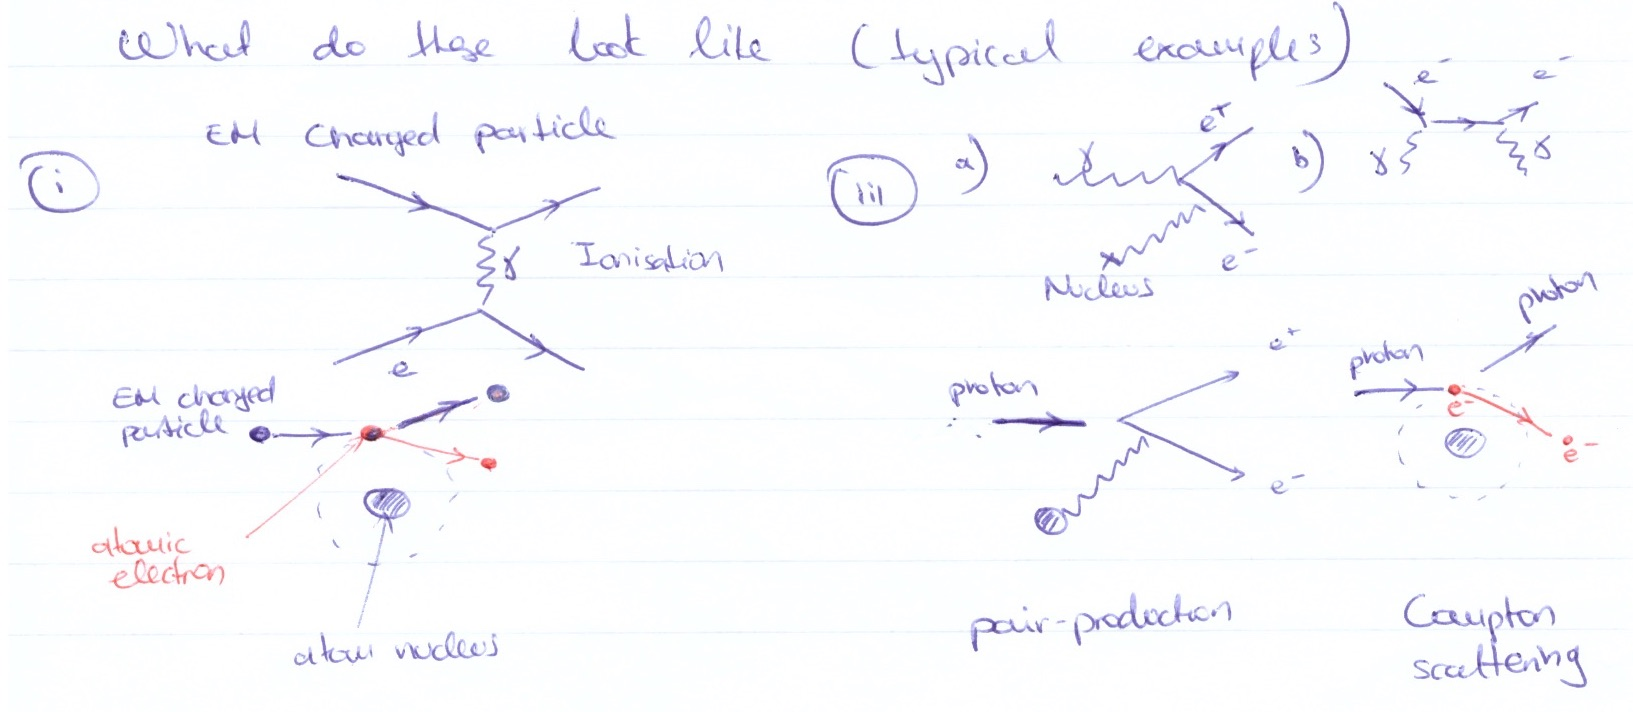
\includegraphics[width=0.95\textwidth]{fig/strongforce/matterinteractions/interactions1.jpg}\newline
%%%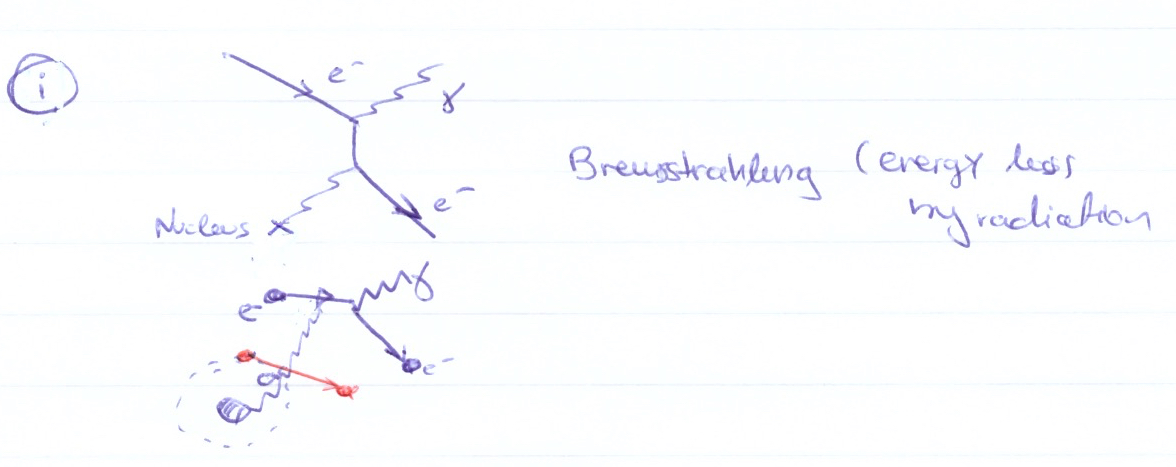
\includegraphics[width=0.8\textwidth]{fig/strongforce/matterinteractions/interactions2.jpg}
%%%\end{center}
%%%
%%%
%%%\subsubsection{Energy loss by ionisation}
%%%We can quantify the energy loss of a particle traversing through the detector, by looking at the average rate of energy lost per unit distance.
%%%
%%%
%%%For an incident particle of charge $ze$ with mass $M>>m_e$, losing energy by ionising atomic electrons in a material with atomic number $Z$ we can use the Bethe-Bloch equation:
%%%
%%%\begin{equation}
%%%\label{eq:bethebloch}
%%%<\frac{dE}{dx}>\approx -2C\frac{m_ec^2Zz^2}{\beta^2A}\rho\left[\frac{1}{2}\log\frac{2m_ec^2\beta^2\gamma^2T_{\rm max}}{I^2}-\beta^2-\frac{\delta(\beta\gamma)}{2}\right]
%%%\end{equation}
%%%with \[C=2\pi N_A\frac{e^2}{4\pi\epsilon_0m_ec^2}.\] 
%%%$I$ is the mean ionisation potential ie $h<\nu_e>$ (given by $\sim10Z$~eV for $Z>20$), $\rho$ is the density of the material, $\delta(\beta\gamma)$ is a density correction term because the incoming particle can polarise the medium, and $T_{\rm max}$ is the maximum energy transfer in a single collision given by
%%%\[
%%%T_{\rm max}=\frac{2m_ec^2\beta^2\gamma^2}{[1+2\gamma m_e/M +(m_e/M)^2].}
%%%\]
%%%For $\frac{\gamma m_e}{M}<<1$, $T_{\rm max}$ can be simplified to
%%%\[
%%%T_{\rm max}\sim2\gamma^2\beta^2m_ec^2.
%%%\]
%%%
%%%\exercise{
%%%One can approximate the picture of a charged particle of mass $M \gg m_e$ with charge $ze$ traversing a material of atomic number $Z$, as an infinitely long cylinder of radius $b$, with charge uniformly distributed  on the surface, surrounding the charged particle which sits in the middle. Let us consider this charged particle interacting with an electron in the medium.
%%%\begin{center}
%%%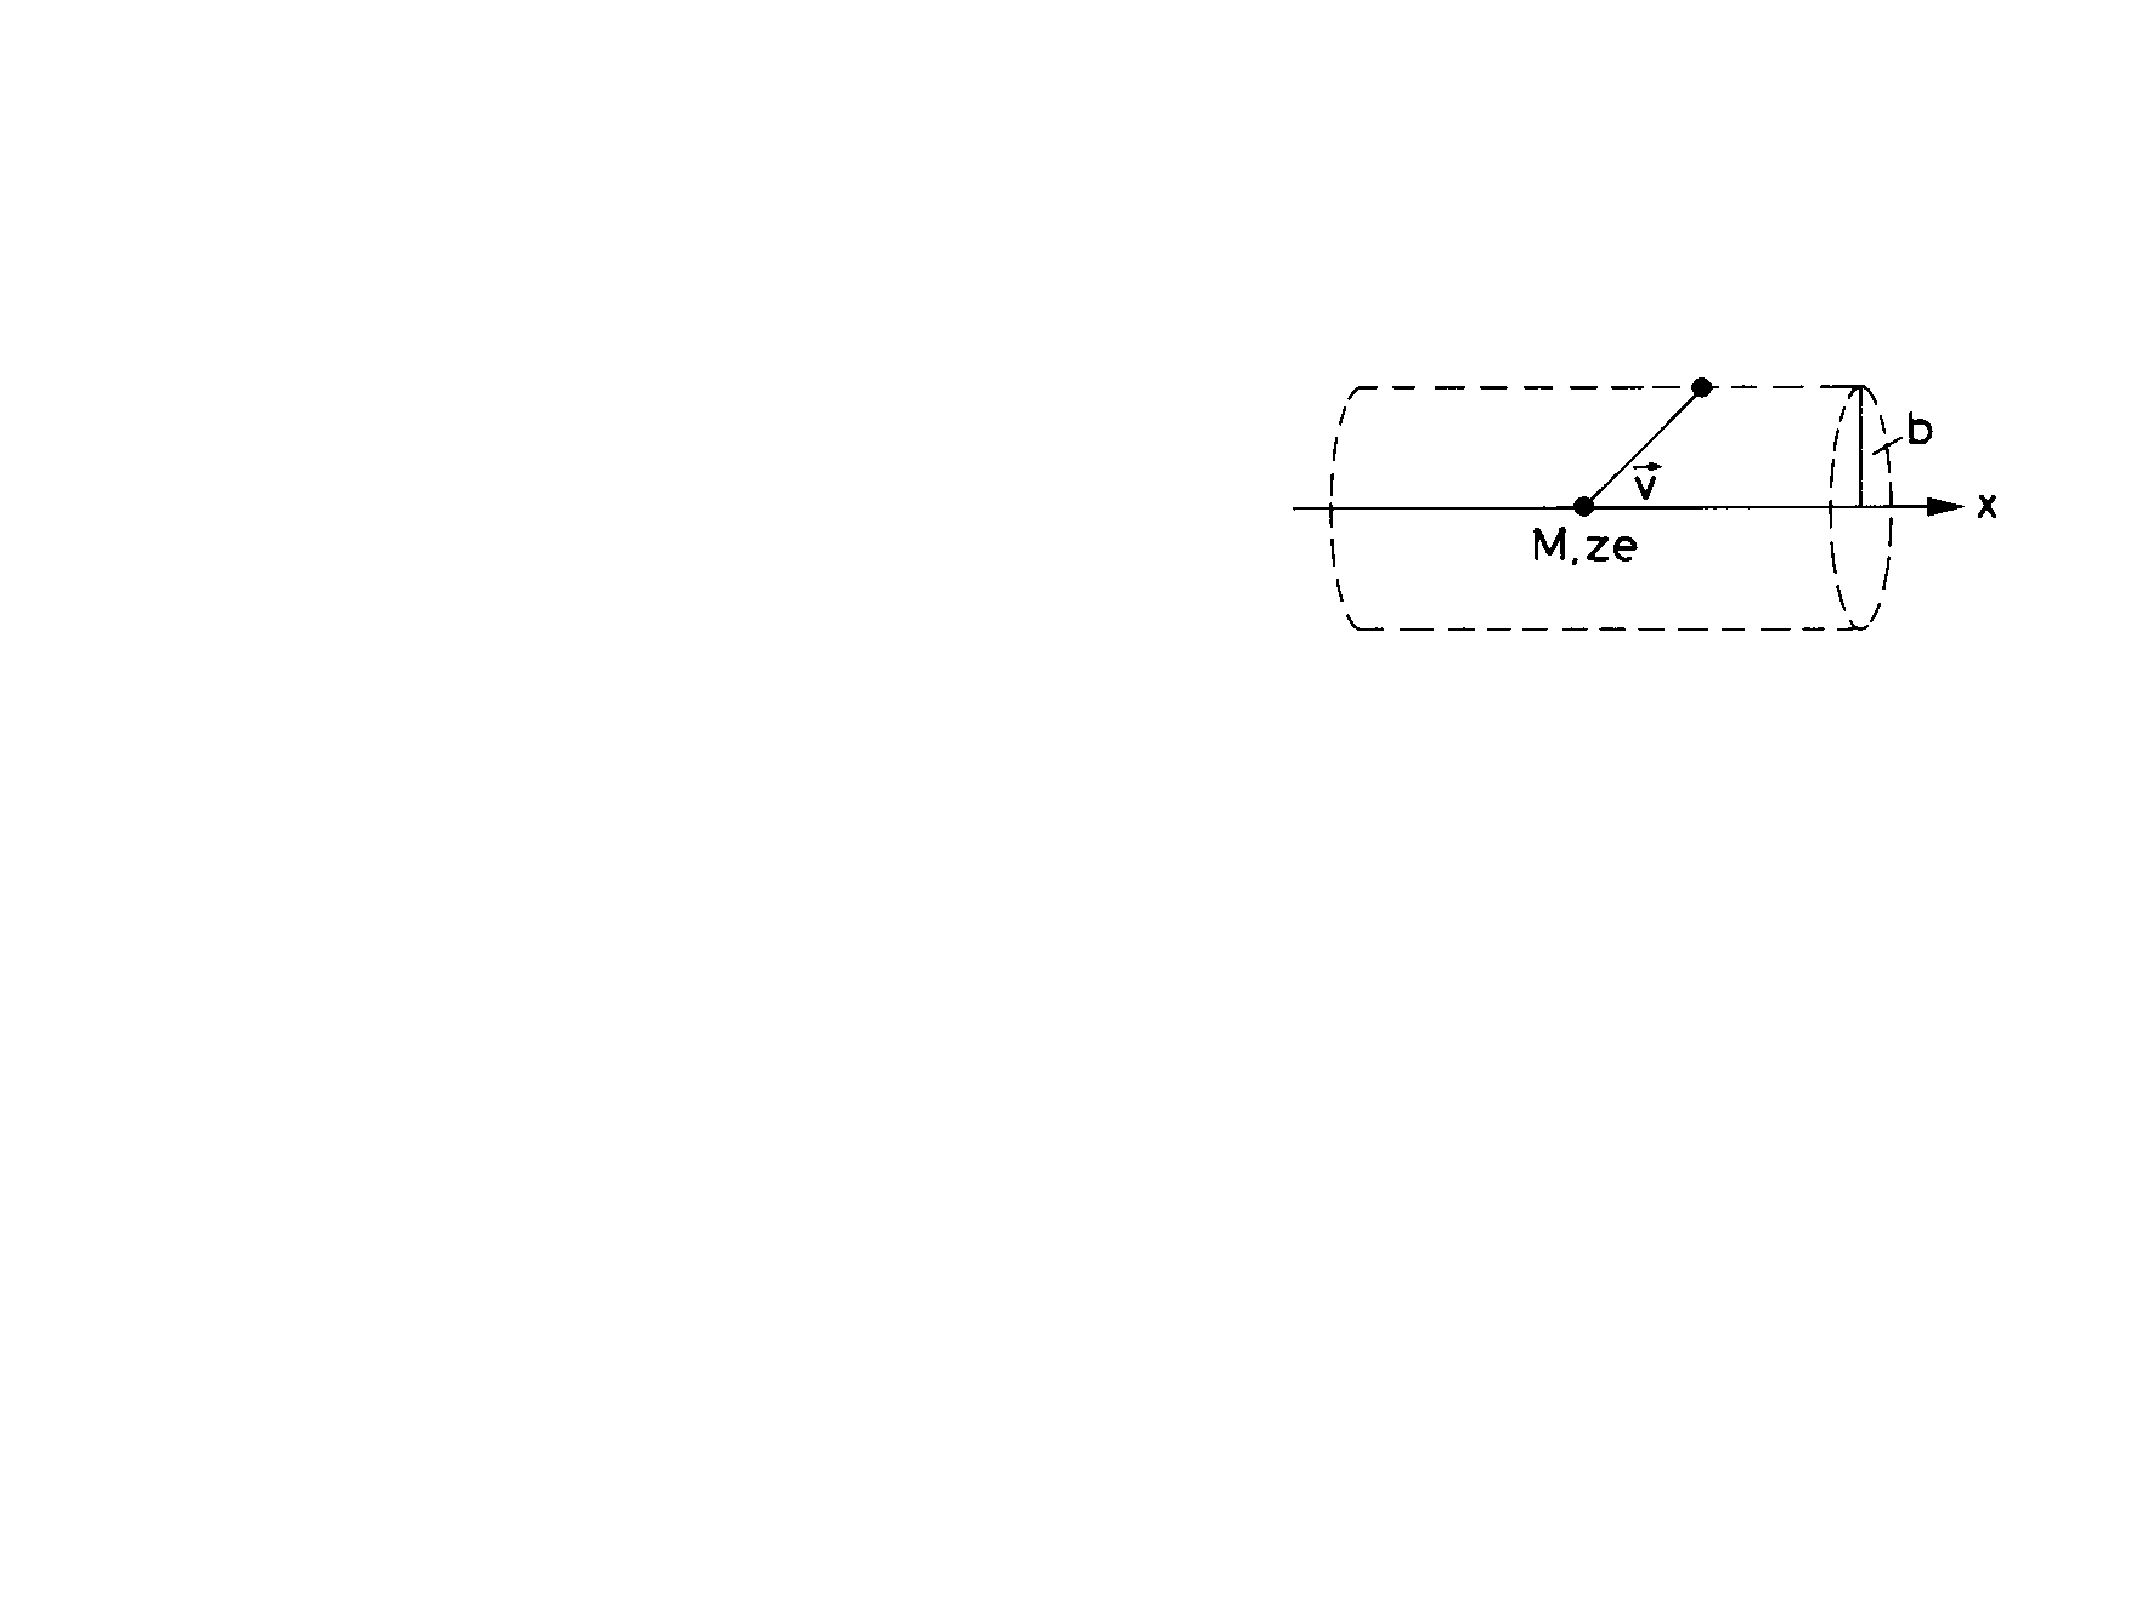
\includegraphics[width=0.5\textwidth]{fig/strongforce/matterinteractions/particle_in_cylinder.pdf}
%%%\end{center}
%%%By applying Gauss's law, show that the momentum transfer perpendicular to the motion of the charged particle, defined by $\Delta p_{\perp}=\int F_{\perp} dt$, is given by $\frac{2ze^2}{bv}$, where $v$ is the speed of the charged particle. Show that $\Delta p_{\parallel}=0$. You can use the fact that in natural units $\epsilon_0=\frac{1}{4\pi}$.\\\\
%%%
%%%Consider now a section of this cylinder of length $dx$. Also let's assume the surface of the cylinder has a width $db$. Show that if the electron density of the cylinder in $n$, the number of electrons contained within this cylinder section is $N_e=n(2\pi b)dbdx$. Therefore show that the energy loss per path length $dx$ traversed by the charged particle is given by:
%%%\[dE=-\frac{4\pi n z^2 e^4}{m_e v^2}\frac{db}{b}dx\]
%%%Hint: Energy transferred onto a single electron on surface of cylinder is given by $\Delta E=\frac{\Delta p^2}{2m_e}$\\\\
%%%
%%%By integrating between $b_{\rm min}$ and $b_{\rm max}$ we have:
%%%\[
%%%\frac{dE}{dx}=-\frac{4\pi n z^2e^4}{m_ev^2}\log\frac{b_{\rm max}}{b_{\rm min}}
%%%\]
%%%The question now is what are sensible values for $b_{\rm min}$ and $b_{\rm max}$. 
%%%If $b$ becomes so large that the energy transfer is lower than the mean energy required to ionise an electron (given by $I=h<\nu_e>$). The minimum value of $b$ occurs when the maximum possible energy transfer occurs. From relativistic energy-momentum conservation, the maximum energy transferred is $\approx 2\gamma^2\beta^2m_e$ (in natural units)
%%%Therefore show that:
%%%$\displaystyle \frac{dE}{dx}=-\frac{4\pi z^2 e^4}{m_e \beta^2}n\frac{1}{2}\log\frac{2m_e\beta^2\gamma^2}{h<\nu_e>}$
%%%}
%%%
%%%\paragraph{Example: Pions in Cu.} Features are common for all materials
%%%
%%%\begin{center}
%%%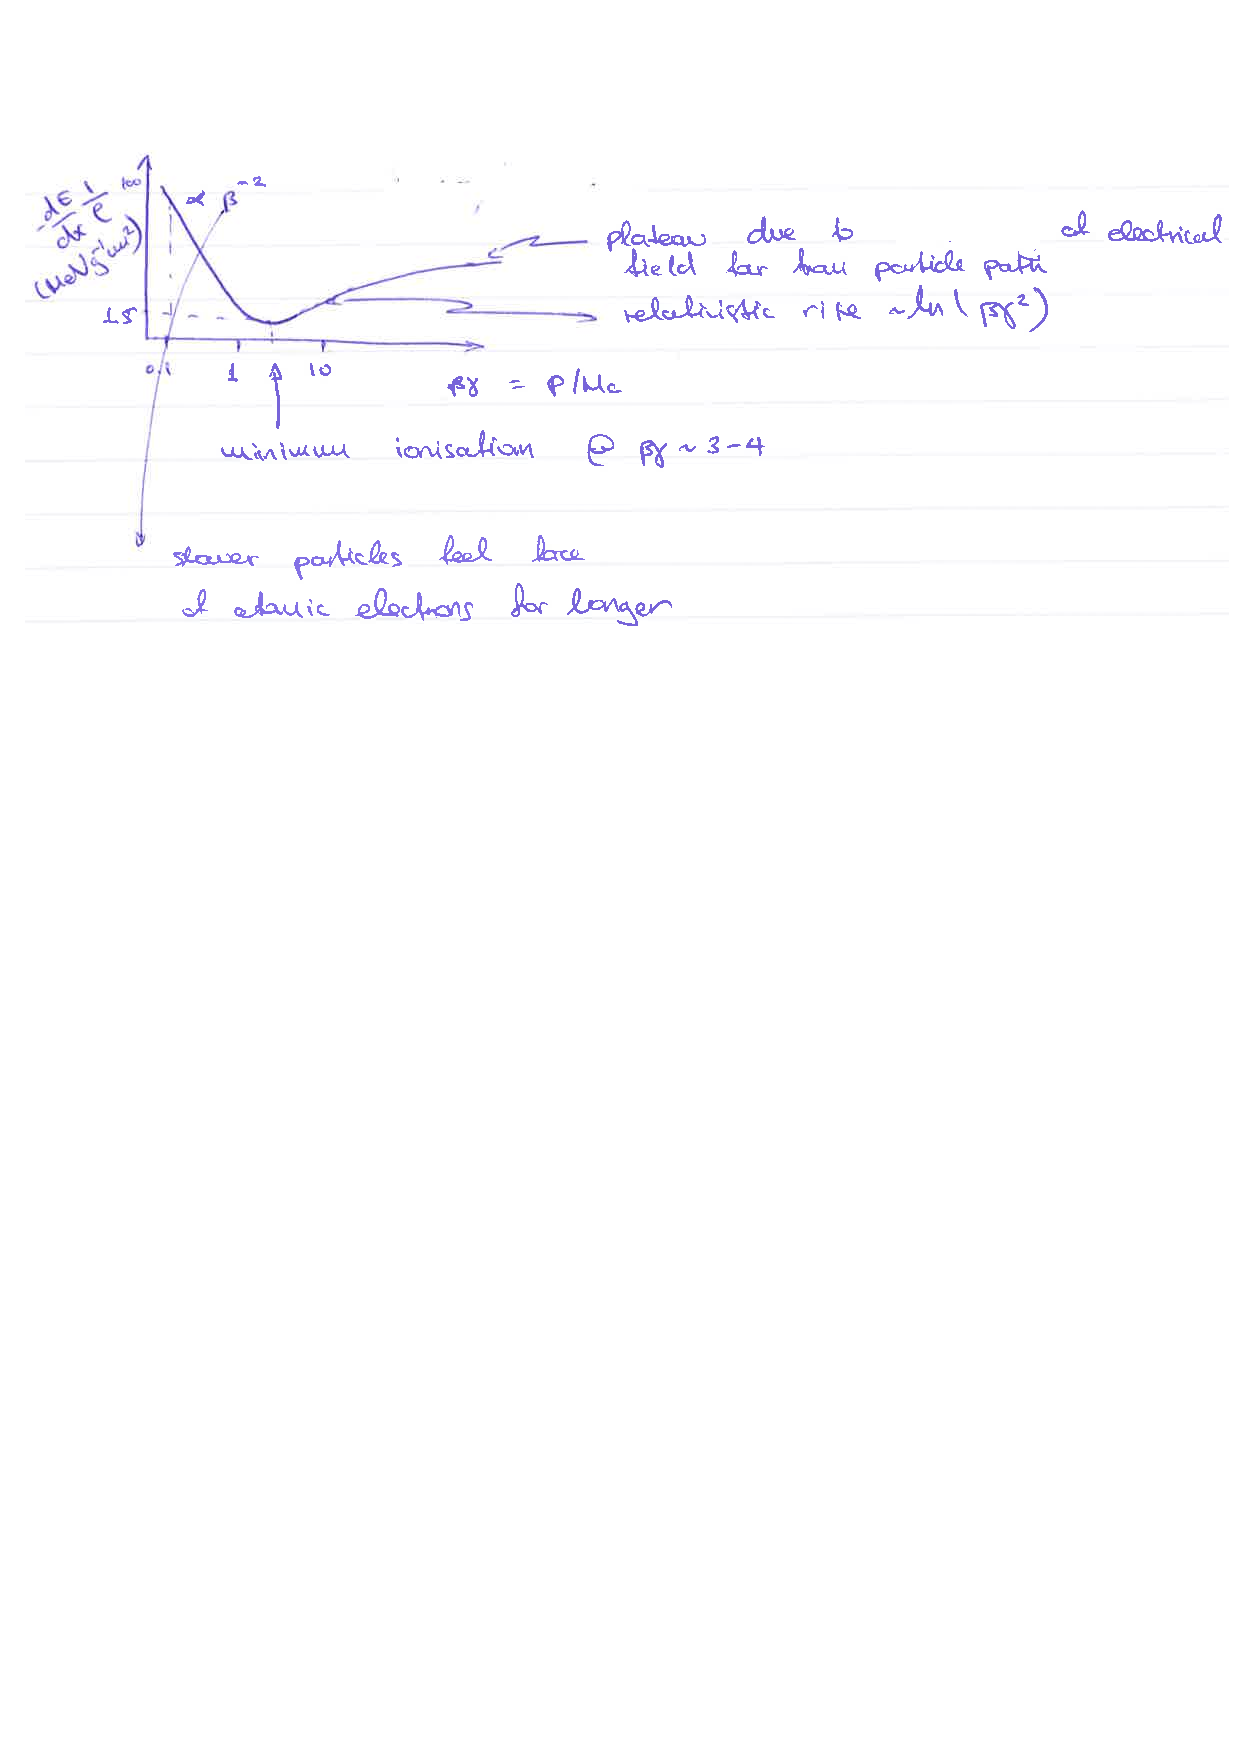
\includegraphics[width=0.95\textwidth]{fig/strongforce/matterinteractions/interactions4.pdf}
%%%\end{center}
%%%
%%%Let us consider some key features, ignoring the $-\beta^2$ and $-\delta(\beta\gamma)$ terms for a moment we have:
%%%\[<\frac{dE}{dx}>\propto -\frac{1}{\beta^2}\log{({\rm const}\cdot\beta^2\gamma^2)}.\]
%%%\begin{itemize}
%%%\item The $1/\beta^2$ fall is due to the fact that slower particles feel the force of atomic electrons for longer. 
%%%\item The $\log{({\rm const}}\cdot\beta^2\gamma^2)$ term is a relativistic rise which comes about due to the fact that high energy particles the electric field transverse to the direction of motion of the particle increases, thus increasing the probability of an interaction.
%%%\end{itemize}
%%%The plateau of the $<\frac{dE}{dx}>$ distribution for $\beta\gamma>10$ is due to the fact that the incoming particle polarises the medium thus shielding the electric field far from the particle path, thus cutting the long range contribution. This is the reason behind the $\delta(\beta\gamma)$ term.  
%%%
%%%The figure below shows the energy lost via ionisation in a sub-detector of ALICE (A Large Ion Collider Experiment) at CERN. It is evident that if one knows the momentum of the incoming particle, then the energy lost through ionisation can distinguish between different incoming particles.
%%%\begin{center}
%%%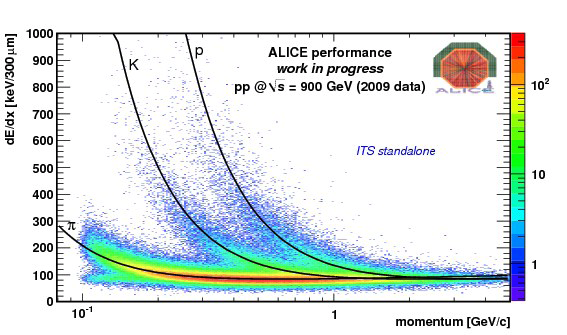
\includegraphics[width=0.95\textwidth]{fig/strongforce/matterinteractions/alice_dedx.png}
%%%\end{center}
%%%
%%%\paragraph{Multiple scattering through small angles: time permitting}
%%%A charged particle traversing a medium feels the Coulomb force of nuclei and hence gets deflected. As it gets multiple deflections from multiple nuclei as it traverses the material, this effect is called ``multiple scattering''. The deflection angle follows a Gaussian distribution centred at zero with a width $\theta_0$ given by:
%%%\[
%%%\theta_0\propto \frac{z\sqrt{x}}{vp}(1+0.038\log{x}+{\rm const})
%%%\]
%%%where $z$ is the charge of the particle in multiples of electric charge, $x$ is the distance travelled, $p$ is the momentum and $v$ is the speed of the particle traversing the medium. A pictorial view of the deflection can be seen below.
%%%
%%%\begin{center}
%%%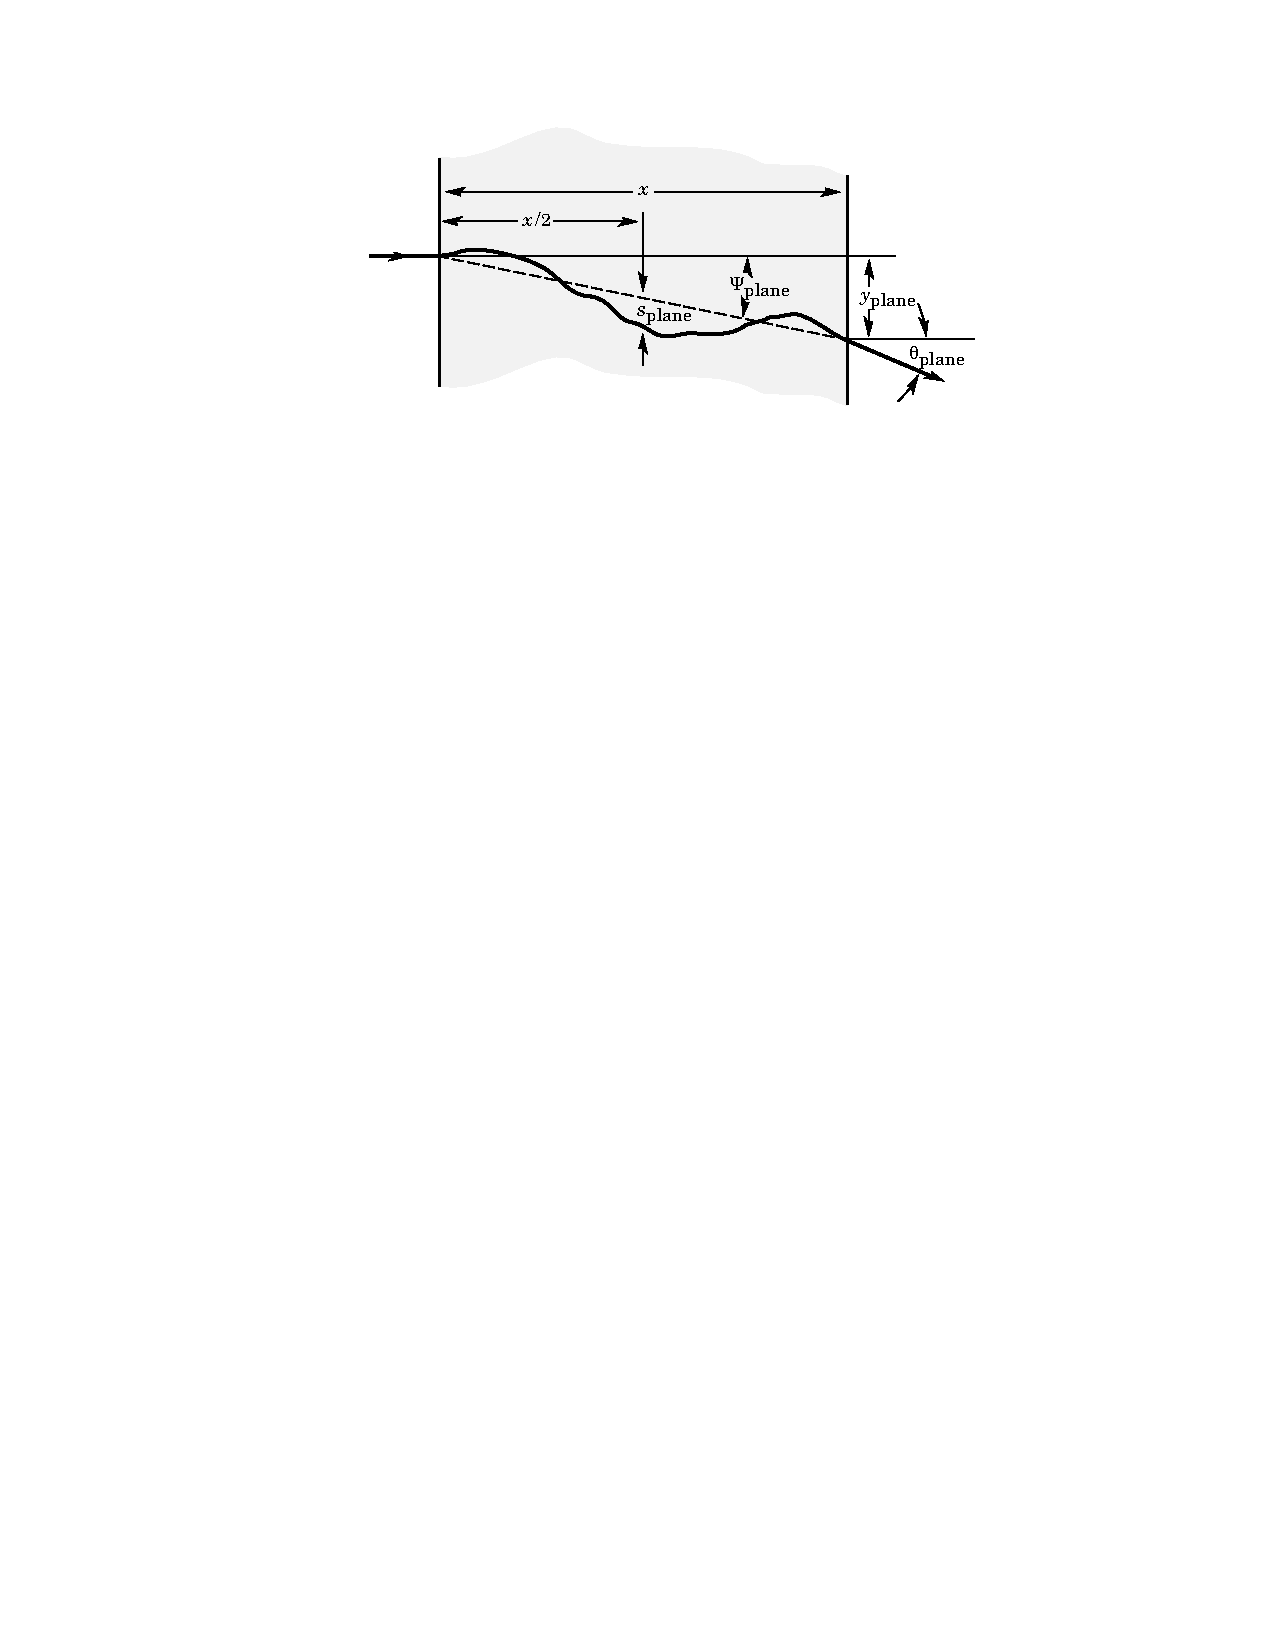
\includegraphics[width=0.95\textwidth]{fig/strongforce/matterinteractions/scattering_angle.pdf}
%%%\end{center}
%%%
%%%
%%%\paragraph{Particle Range: time permitting}
%%%The range $R$ of a particle is defined as the distance it will travel
%%%in the material before loosing all its energy through ionisation. It is a useful
%%%quantity, however it is not the full picture as particles can loose energy through
%%%other means, as we shall see later in the course.
%%%In any case it is interesting to calculate. 
%%%Suppose a particle enters a material with energy $E_0$. We can therefore define the range as
%%%\[
%%%<R>=\int_{E_0}^{0}\frac{dE}{<dE/dx>}.
%%%\]
%%%Insterting Eq.~\ref{eq:bethebloch}, we get 
%%%\begin{equation}
%%%<R>\propto \frac{E_{0}^{3/2}}{\sqrt{m}}.
%%%\end{equation}
%%%For the case when energy of incoming particle larger than the rest mass we have
%%%\[
%%%<R>\propto (\gamma m v)^{3/2}.
%%%\]
%%%
%%%\fbox{\parbox{0.98\textwidth}{
%%%\paragraph{Beyond scope:}
%%%So far we have discussed the average energy loss through ionisation $<\frac{dE}{dx}>$. In fact the actual energy loss scatters around the mean value ie
%%%\begin{center}
%%%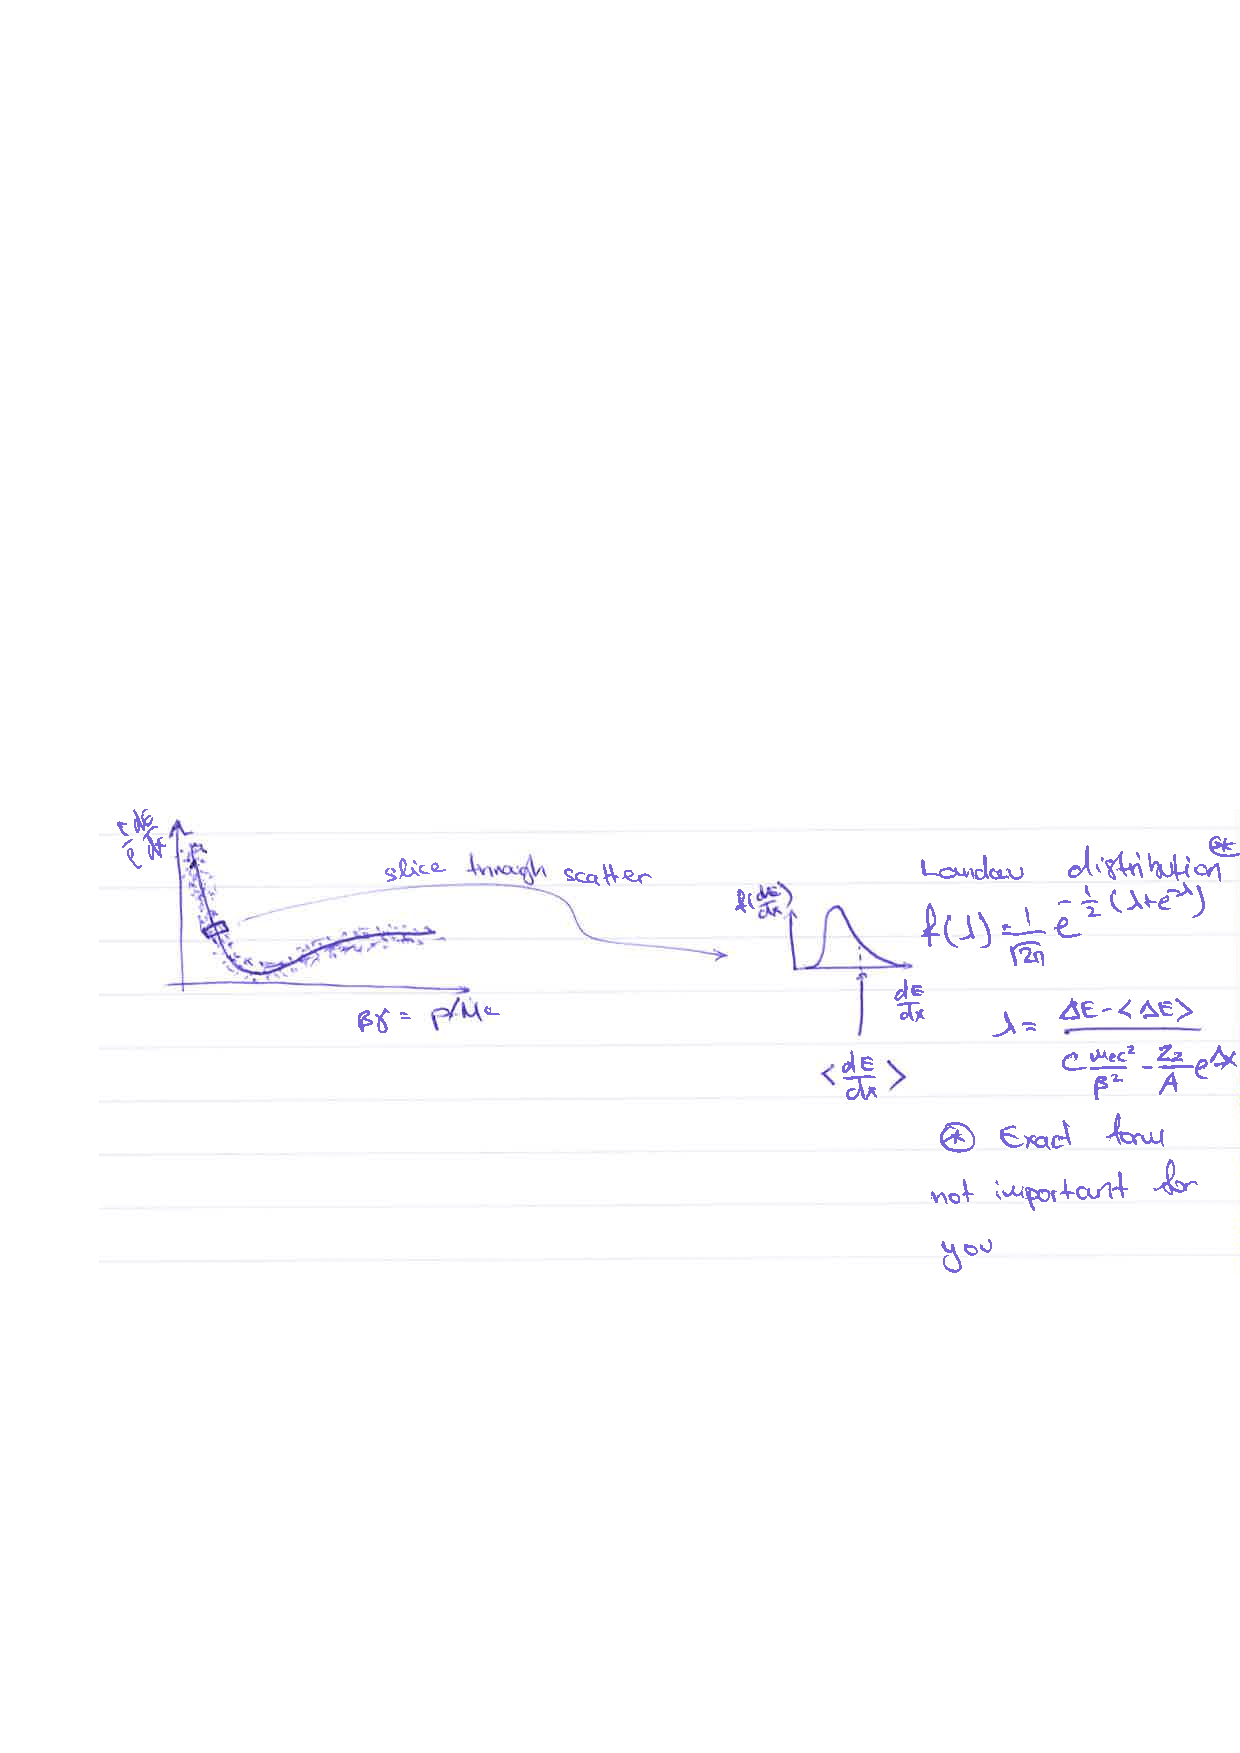
\includegraphics[width=0.95\textwidth]{fig/strongforce/matterinteractions/interactions3.pdf}
%%%\end{center}
%%%
%%%
%%%}}

